

\chapter{Herstellung und Zusammenbau}
\label{chap:herstllung}

\section{Herstellungsprozess der Komponenten}
\subsection{Skelett und grundlegende Bootsform}
Da für dieses Projekt keine computergesteuerte \ac{cnc} Fräse zur Verfügung steht, werden die Spanten des Bootes mittels einer elektrischen Handstichsäge aus drei verleimten Tannenbrettern mit den Massen 240 mal 40 cm und einer Stärke von 18 mm ausgesägt. Dafür werden die Baupläne der zehn Elemente mithilfe eines Plotters im Massstab 1:1 ausgedruckt und  mit Hilfe von transparentem Backpapier mittels der Abpausmethode auf Tannenholzbretter übertragen, und anschliessend mit der Handstichsäge ausgesägt.

Die Erstellung der Spanten erfolgt in zwei Arbeitsschritten. Im ersten Schritt wird die äussere Form ausgesägt. In einem zweiten Schritt wird danach Material innerhalb der Elementen entfernt. Dies wird aus Gewichtsgründen gemacht und schafft den für die spätere Montage der Elektronik und der Energieversorgung notwendigen Freiraum im Inneren des Bootes.

An den entsprechenden Stellen an der Oberseite der Spanten werden je zwei Löcher gebohrt und die Elemente werden dann mit Hilfe von zwei Aluminiumrohren verbunden. Um eine Verschiebung der Elemente während des Herstellungsprozess zu vermeiden, werden diese mit Heisskleber mit den Aluminiumrohren verklebt. 
\begin{figure}[H]
    \centering
    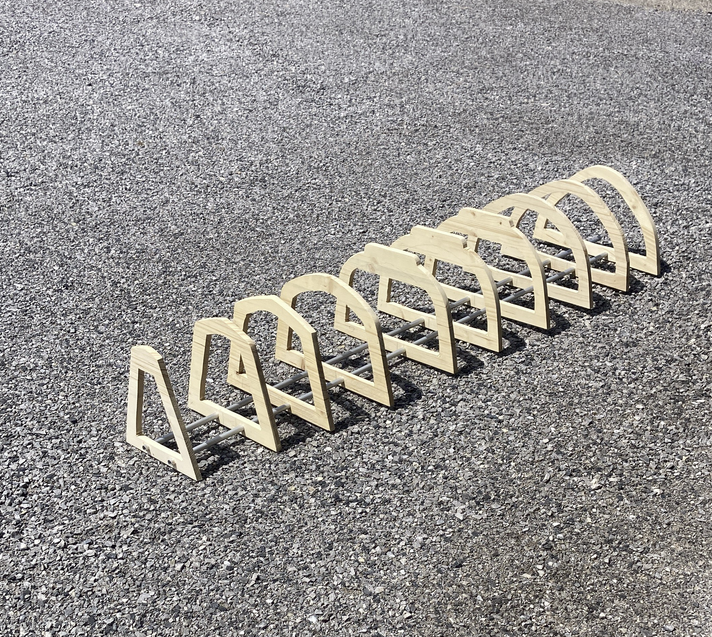
\includegraphics[width=1\linewidth]{rippe1.png}
    \caption{Rippenförmige Anordnung der Tragelemente}
    \label{fig:enter-label}
\end{figure}

Da die Spanten  mit einer Handstichsäge ausgesägt werden, lassen sich  Ungenauigkeiten nicht völlig vermeiden. Daher weichen die tatsächlichen Masse der Spanten bis zu 5 mm von den Planwerten ab. Obwohl dies eine relative Abweichung ist, kann der Fehler in den folgenden Arbeitsschritten ausgebessert werden. 

Da für die Elemente aus Kostengründen kein Massivholz genommen werden kann, muss auf Leimholz zurückgegriffen werden. Dies hat zum Nachteil, dass einzelne Elemente einen Bruch erleiden, wenn zu viel Druck auf die geleimten Stellen wirkt. Beschädigte Elemente werden nicht verwendet, sondern durch neu  erstellte Kopien ersetzt. 
\begin{figure}[H]
    \centering
    \includegraphics[width=0.25\linewidth]{bruch.png}
    \caption{Bruch eines Elements}
    \label{fig:bruch}
\end{figure}

Im Anschluss wird eine Schicht Balsaholz über die Rippen gelegt. Die verwendeten Balsaholzbrettchen haben eine Stärke von 1mm und sind 100 cm lang. Zur Befestigung an den Spanten wird eine Tackerpistole verwendet. Durch Verspannungen im Holz ergeben sich unglücklicherweise kleinere Verformungen, welche sich negativ auf die endgültige Bootsform auswirken können.

\subsection{Glasfaserbeschichtung}
Um eine robuste  Aussenhülle für das Boot zu schaffen, wird eine glasfaserverstärkte Epoxidharzschicht  aufgetragen. Die Verbindung von Glasfasermatten mit Epoxidharz ergibt eine äusserst harte und stabile Schicht.  Dafür  werden die Glasfasermatten auf die Balsaholzplanken gelegt und mit Epoxidharz bestrichen. Dies führt dazu, dass die Epoxidschicht die Form des Bootes annimmt. Das unterliegende Balsaholz bildet also  die formgebende, und die Glasfaser-Epoxidschicht die  strukturgebende Komponente. 

Dieses Vorgehen führt jedoch auch zu Problemen, da der Auftrag der Glasfaser-Epoxidschicht zu Verspannungen in der Balsaholzschicht führt. Auch die Schwankungen der Feuchtigkeit in der Werkstatt bewirken Verspannungen, welche sich dann ebenfalls auf die Balsaholzschicht auswirken.  Um diese Dellen in der Aussenhülle auszugleichen, muss sehr viel Expoxidspachtelmasse aufgetragen wird. Dafür wird eine Mischung von Expoixid und entsprechendem Härtungsmittel verwendet.  Um das folgende Planschleifen der Oberfläche zu vereinfachen, werden diesem Gemisch Microballons beigemischt und ein Tixotropiermittel wird zugegeben, um das Gemisch einzudicken. Der Prozess des Auftragens und Abschleifens muss  viele Male wiederholt werden. Das ist sehr zeitaufwändig, da immer gewartet werden muss, bis die neu aufgeragenene Schicht vollständig getrocknet ist.  Dabei wird  versucht einen möglichst glatten, stromlinienförmigen Körper zu formen.

Um eine Asymetrie beim Bug zu vermeiden, wird sehr viel \\Expoxid-Spachtelmasse augetragen. Kleine Glasfaserschnippsel, welche zur Spachtelmasse dazugerührt werden, geben dieser weitere Stabilität, damit der Bug gut geschützt ist.

Zum Schluss wird der Bootskörper mit Sperrholzplatten abgedeckt. Diese werden in einem ersten Schritt auf den offenen Bootskörper gelegt. Dann werden mit einem Bleistift die Konturen des Bootskörpers nachgezogen. Die Deckplatten werden entlang der Bleistiftmarkierungen ausgesägt. In der Mitte des Boots wird eine Öffnung in die Deckplatten gesägt und die Deckplatten mit dem Schiffskörper verleimt. Die vorhandene Lücke im Deck wird erst nach dem Einbau des Masts und der Elektronik und der Bemalung der Deckplatte mit einer weiteren, abnehmbaren Sperrholzplatte verschlossen. Am Schluss werden noch die Positionslampen angebracht. 
\subsection{Ruder}
Das Ruder wird aus einer Tannen-Leimholz Platte ausgesägt. Dabei wird daselbe Verfahren wie bei den Spanten angewendet. Anschliessend wird das Werkstück mit der Schleifmaschine bearbeitet und in Form gebracht. 
\begin{figure}[H]
    \centering
    \includegraphics[width=0.5\linewidth]{assets/ruderimagegrafik.png}
    \caption{Fertiger Einbau des Ruders}
    
\end{figure}

Nach der Lackierung mit roter Farbe wird das Ruder am Heck des Schiffskörpers befestigt und mit der Welle des Aktuators verbunden.
\subsection{Kiel}
In einem ersten Schritt werden die 5 Bretter ausgesägt, miteinander verleimt und verschraubt. Anschliessend werden in die Löcher für die Gewindestangen in die beiden äusseren Kielbretter gebohrt. 

Im nächsten Schritt wird ein Loch in jedes der beiden 2 Kg Gewichte gebohrt. So können die Gewichte mit dem Kielhauptbrett verschraubt werden. Nach dem Druck der beiden Schutzgehäuse werden diese über die Gewichte gestülpt und mit dem Kielhauptbrett verleimt.    
\begin{figure} [H]
    \centering
    \includegraphics[width=0.3\linewidth]{assets/Kiel_lakiert.png}
    \caption{Fertiger Kiel}
    \label{fig:enter-label}
\end{figure}

\subsection{Segel}
Das Segel besteht aus EPS und setzt sich aus vier identischen Teilen zusammen, die aus EPS-Platten ausgeschnitten werden. Je zwei Platten bilden die rechte und die linke Seite des Segels, das eine aerodynamisch günstige Form aufweist. Dazu werden die beiden Segelhälften verklebt.  
\subsubsection*{EPS Schneidegerät}
Mit speziellen Schneidegeräten können Formen aus EPS Platten geschnitten werden. Konventionelle EPS Schneidgeräte sind allerdings nicht genügend gross, um die vier Teile auszuschneiden, weshalb ein eigenes Schneidegerät gebaut werden muss. Alle EPS Schneidegeräte funktionieren nach demselben Prinzip. Dabei wird ein Metalldraht  auf  60$^\circ$ C - 100$^\circ$ C erhitzt und ins EPS gefahren, wo dieses lokal zum Schmelzen gebracht wird. Indem der Draht durch den EPS Körper gezogen wird, entsteht ein sauberer Schnitt. Der Draht wird dadurch erhitzt, dass an ihm eine elektrische Spannung gelegt wird. Der Draht bildet einen Widerstand und wird heiss. Der Draht ist so ausgelegt, dass er einen möglichst hohen Wiederstand aufweisst. 
Damit die  vier grossen Segelteile als ganzes aus EPS Blöcken geschnitten werden können, wird ein eigenes einfaches Schneidegerät mit entsprechenden Dimensionen gebaut.  Dazu wird ein sogenannter \enquote{Widerstandsdraht} mit einem Durchmesser von $\varnothing$ 0.2mm gekauft. Dieser wird dreifach verdrillt und daraus ein Schneidedraht mit einer Länge von 1.5 m erstellt. Die beiden Enden werden in einen U-förmigen Rahmen aus Tannenholzlatten gespannt. Als Stromquelle dient zunächst ein Labornetzteil, das 3A bei 12V liefert. 

Die ersten Versuche, zunächst noch mit einem einfachen und anschliessend mit einem zweifachen Draht, verlaufen erfolglos. Erst als eine, dreifach verdrillter Draht und ein stärkeres Labornetzteil, das 5A bei 12 V liefert, verwendet wird, wird der Draht soweit aufgeheizt, dass damit EPS geschnitten werden kann.     
\begin{figure}[H]
    \centering
    \includegraphics[width=0.5\linewidth]{foamcutter1.png}
    \caption{Foamcutter}
    \label{fig:enter-label}
\end{figure}
\subsection*{Grosssegel}
Um die geplante Form aus den \ac{eps} Platten schneiden zu können, wird zuerst mithilfe eines Lasercutters eine Halbprofilform aus Sperrholz erstellt. Je eine solche Halbprofilform wird mit zwei  Schrauben an den beiden kürzeren Seiten einer EPS Platte  befestigt. Der heisse Schneidedraht kann damit entlang der Kante der Halbprofilschablone durch den EPS Block gezogen werden. So entsteht ein halbes Segel mit der Form der Halbprofilschablonen. \\


\begin{figure}[H]
    \centering
    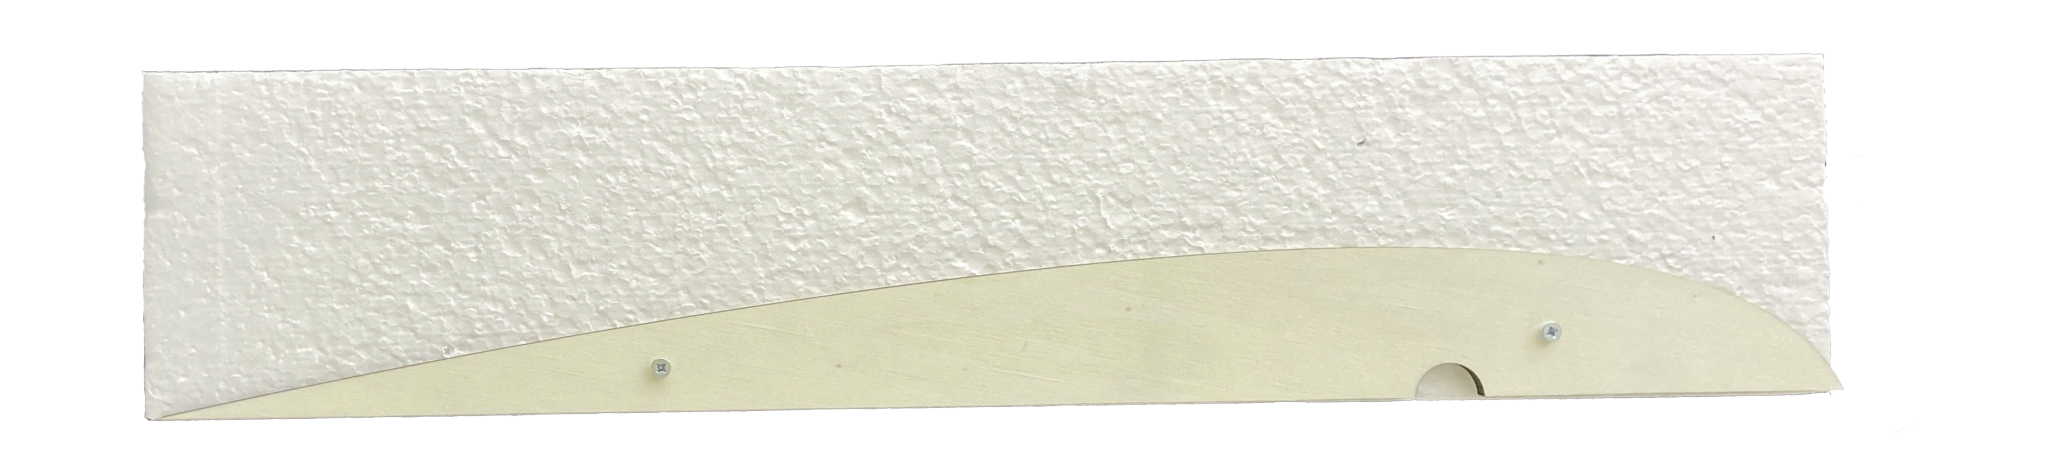
\includegraphics[width=1\linewidth]{assets/template_on_foam.png}
    
    \caption{Seitenansicht eines Elements mit der Schablone}
    \label{fig:enter-label}
\end{figure}

Anschliessend muss auf der planen Seite des Halbsegelteils noch eine halbrunde Kerbe ausgeschnitten werden. In ihr findet bei der Verleimung der Platten der Aluminiummast Platz. Nicht jeder Schneideversuch verläuft erfolgreich. Wenn die beiden Enden des Schneiddrahtes nicht synchron über die Halbprofilform geführt werden, oder wenn dieser nicht präzis gefolgt wird, weist der ausgeschnittene Körper erhebliche Formfehler auf. Auch bei einem an sich erfolgreichen Schnitt ergeben sich aber kleine Ungenauigkeiten, die aber mit einem Schliff des Bauteils korrigiert werden können. 

Nachdem erfolgreich vier Profile ausgeschnitten worden sind, wird der Mast in die ausgesparte Kerbe gelegt und fixiert. Danach werden die vier Profile in Paaren verklebt. Im Bootskörper sind zwei Halterungen für den Mast vorgesehen, die ein Kugellager enthalten. Der Mast wird durch deren Öffnungen gesteckt und am Schluss in den Schleifring gesteckt.
\subsection{Sailflap}
Das Sailflap wird mit derselben Technik wie das Grosssegel hergestellt. Zu seiner Befestigung werden zwei Carbonstäben verwendet, die am Grosssegel fixiert werden. Am unteren Stab wird der Aktuator befestigt, bevor das Sailflap mit den Carbonstäben fixiert wird. Zum Abschluss wird das Sailflap an der Welle des Aktuators befestigt.   
\section{Bemalung}
Da das autonome Segelboot gut sichtbar sein soll, wird es in roter Signalfarbe bemalt. Dazu wird seidenmatter Acryllack verwendet, der mithilfe einer Farbwalze auf den Bootskörper aufgetragen wird. Es wurde bewusst  eine matte Farbe  gewählt, da diese kleine Ungenauigkeiten und Dellen in der Bootsform besser kachiert als glänzende Farben. 

Da das Ruder, der Kiel und das Deck keine Schützhülle aus glasfaserverstärktem Epoxidharz verfügen, hat die Farblackierung bei diesen Bauteilen auch eine Schutzfunktion.

Erst wenn die Farbe trocken ist, wird am Bug der Schiffsname Panta Exo aufgemalt. Dazu wird eine Schablone erstellt und verwendet. 
\section{Einbau der Elektronik}
Als erstes wird ein digitaler Schaltplan mit allen Sensoren und Aktuatoren und Sensoren erstellt. Dieser dient als Bauanleitung für den Bau. Die für die Erstellung des Schaltplans notwendigen Informationen werden den Datenblättern der Geräte und  Sensoren entnommen, in welchen ihre Funktionsweise beschrieben und die Betriebsweise erläutert wird.
\subsection{Raspberry Pi}
Der Rasbperry Pi Zero W 1.1 wird in einer kleinen Plastikbox festgemacht und dieses im Schiffskörper zwischen den Spanten 5 und 6 befestigt.
\subsection{Sensoren}
Das GPS Modul, sowie der Gyro und Magnetometer wird wie der Raspberry Pi Zero W 1.1 zwischen den Spanten 5 und 6 platziert. Der Windrichtungssensor wird zuvordest auf dem Deck beim Bug plaziert. Dazu wird seine Grundplatte mit der Deckplatte verleimt. Durch ein kleines Loch im Deck, das unter der Deckplatte des Windrichtungsmesses gebohrt wird, werden dessen Kabel in den Rumpf hinein und dann  nach hinten zum Raspberry Pi Zero W 1.1 geführt.
\subsection{Aktuatoren}
Der Aktuator für das Ruder wird am Heck des Bootes am Achtersteve befestigt. Senie Welle wird mit dem Ruder verbunden. Das Ruder kann bis zu einem Winkel von etwa 60 Grad eingeschlagen werden.
Der Einbau des zweite Aktuators wird oben beim Bau des Sailflap beschrieben. Seine Steuerkabel werden durch das Gosssegel in den Mast und von dort durch den Schleifring in den Bootskörper geführt.  
\subsection{Energieversorgung}
Da der Akku relativ schwer ist, wird er zwischen den Spanten 6 und 7, also ziemlich genau am Längsschwerpunkt des Bootes, platziert und am Boden des Bootsrumpfs befestigt. Da er unter der Wasserliniezu liegen kommt, wird damit die Stabilität des Bootes gefördert. Das Solarpanel wird auf dem Deck vor dem Segel befestigt. Dazu werden die Ösen des Panels von Hacken festgehalten, die in der Deckplatte verschraubt werden.
